\documentclass{article}
\usepackage[margin=0.5cm]{geometry}
\usepackage{polski}
\usepackage[utf8]{inputenc}
\usepackage{graphicx}

\title{Wyniki}
\author{Bartosz Rzepkowski}
\date{March 2020}

\begin{document}

\maketitle

\section*{Legenda}

W trakcie pracy nad tymi wynikami zmieniłem sposób generowania zbioru uczącego sieci. Wcześniej procedura generowania takiego zbioru wyglądała następująco:
\begin{itemize}
	\item wygeneruj losowy, znormalizowany wektor $|\psi_0\rangle$,
	\item znajdź wektor poddany bardzo krótkiej ewolucji czasowej (np. 0.1 jednostek czasu) $|\psi_t\rangle$,
	\item dodaj oba wektory do zbioru uczącego (pierwszy jako wektor wejściowy a drugi jako oczekiwany wyjściowy).
\end{itemize}

Teraz generowanie tego zbioru wygląda następująco:
\begin{itemize}
	\item wygeneruj losowy, znormalizowany wektor $|\psi_0\rangle$,
	\item znajdź wektor poddany bardzo krótkiej ewolucji czasowej (np. 0.1 jednostek czasu) $|\psi_t\rangle$,
	\item dodaj oba wektory do zbioru uczącego (pierwszy jako wektor wejściowy a drugi jako oczekiwany wyjściowy),
	\item zamiast generować kolejny wektor losowy przeprowadź krótką ewolucję wektora $|\psi_t\rangle$ uzyskując wektor $|\psi_{2t}\rangle$ i ponownie dodaj te dwa wektory do zbioru uczącego,
	\item powtórz powyższy krok aż do momentu uzyskania całkowitego porządanego czasu ewolucji. Tzn. np. dla kroku (\textit{t}) długości 0.1 i czasu całkowitego (\textit{t\_total}) równego 10 jednostek czasu wykonalibyśmy 100 takich operacji: 
	$|\psi_{0}\rangle, |\psi_{t}\rangle, |\psi_{2t}\rangle, ..., |\psi_{100t}\rangle = |\psi_{t\_total}\rangle$,
	\item dopiero po zakończeniu opwyższej procedury wygeneruj kolejny wektor losowy.
\end{itemize}

Na samym końcu w obu przypadkach wykonywałem "przetasowanie" zbiorów uczących. Czyli w najnowszej wersji sieć nie uczyła się na występujących bezpośrednio po sobie kolejnych krokach ewolucji, tylko raczej na losowo wybranych jej momentach.



\section{Szukanie dobrego rozmiaru zbioru uczącego (2 warstwy, Adamax, mean squared error, tanh)}

W tej sekcji szukałem najlepszego możliwego rozmiaru zbioru uczącego dla nowego sposobu uczenia sieci. Oznaczenie "training\_set\_size: 1000" oznacza wygenerowanie 1000 wektorów losowych. Jednak docelowo cały zbiór uczący ma 100 000 elementów, ponieważ dla każdego losowego wektora do zbioru dodajemy 100 kolejnych kroków jego ewolucji.

Wlewej kolumnie oznaczonej jako \# zawarto liczbę wektorów losowych generowanych w trakcie tworzenia zbioru uczącego. Wartość w nawiasie w tej kolumnie oznacza precyzję sieci dla JEDNEGO kroku ewolucji (czyli w naszym przypadku dla kroku = 0.1).


\begin{tabular}{|c|c|c|c|} \hline
     \# & Overlap & Korelacja & Współczynnik  \\ \hline
     1000 \\ (0.992) &
     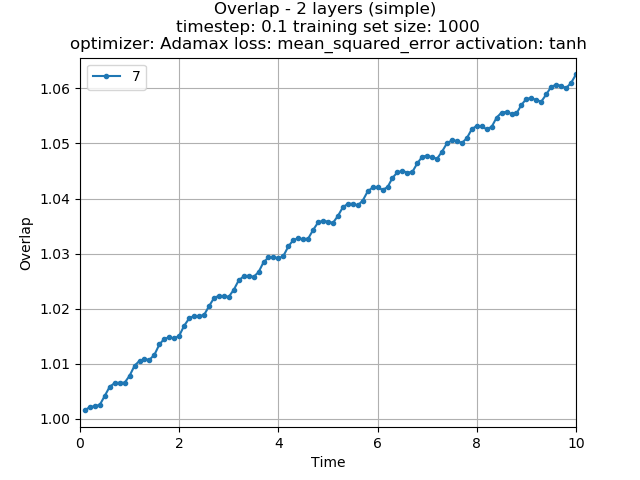
\includegraphics[scale=0.37]{./Searching_for_good_train_set_size/2_layers_simple_train_samples=1000_timestep=0.1_t_total=10.0_optimizer=Adamax_loss=mean_squared_error_activation=tanh/Overlap.png} &
     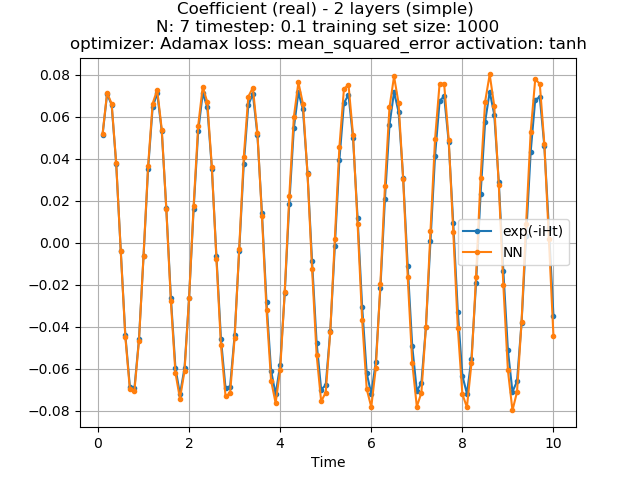
\includegraphics[scale=0.37]{./Searching_for_good_train_set_size/2_layers_simple_train_samples=1000_timestep=0.1_t_total=10.0_optimizer=Adamax_loss=mean_squared_error_activation=tanh/Coeff_N=7_(real).png} &
     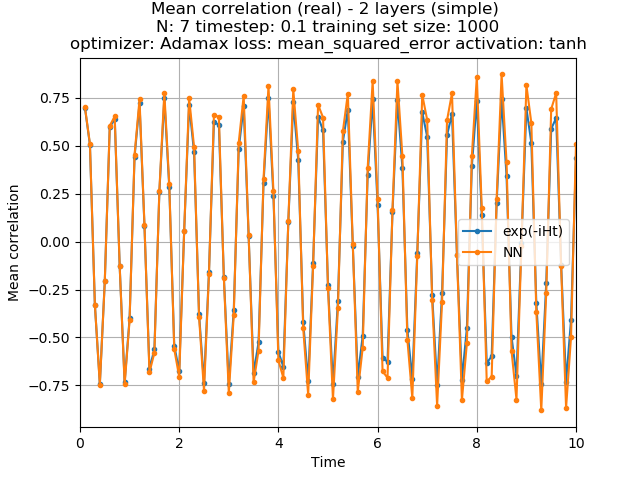
\includegraphics[scale=0.37]{./Searching_for_good_train_set_size/2_layers_simple_train_samples=1000_timestep=0.1_t_total=10.0_optimizer=Adamax_loss=mean_squared_error_activation=tanh/Corr_N=7_(real).png} \\ \hline

\end{tabular}

\begin{tabular}{|c|c|c|c|} \hline
     2000 \\ (0.990) &
     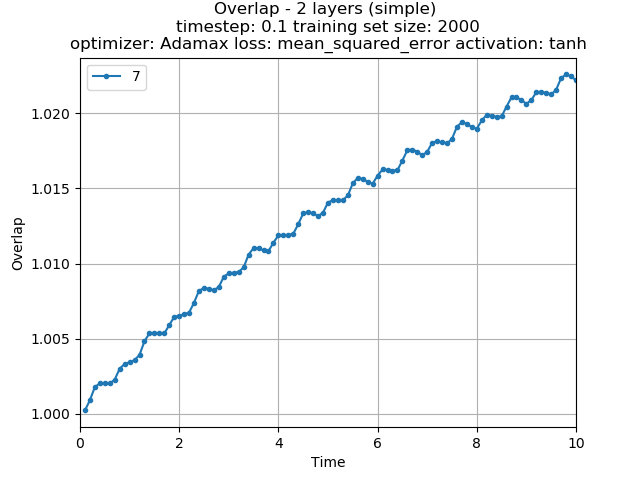
\includegraphics[scale=0.37]{./Searching_for_good_train_set_size/2_layers_simple_train_samples=2000_timestep=0.1_t_total=10.0_optimizer=Adamax_loss=mean_squared_error_activation=tanh/Overlap.png} &
     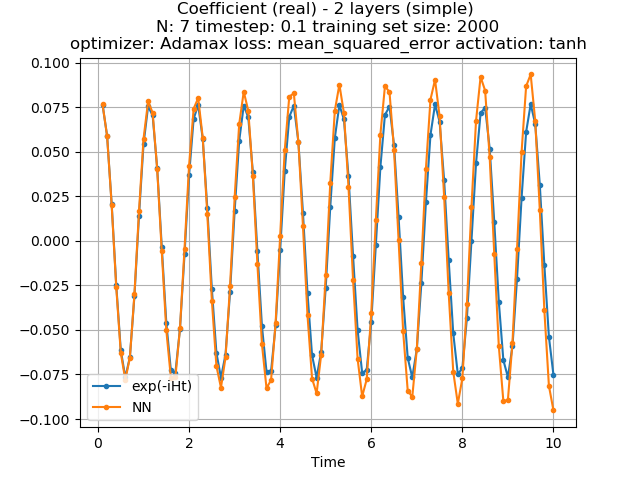
\includegraphics[scale=0.37]{./Searching_for_good_train_set_size/2_layers_simple_train_samples=2000_timestep=0.1_t_total=10.0_optimizer=Adamax_loss=mean_squared_error_activation=tanh/Coeff_N=7_(real).png} &
     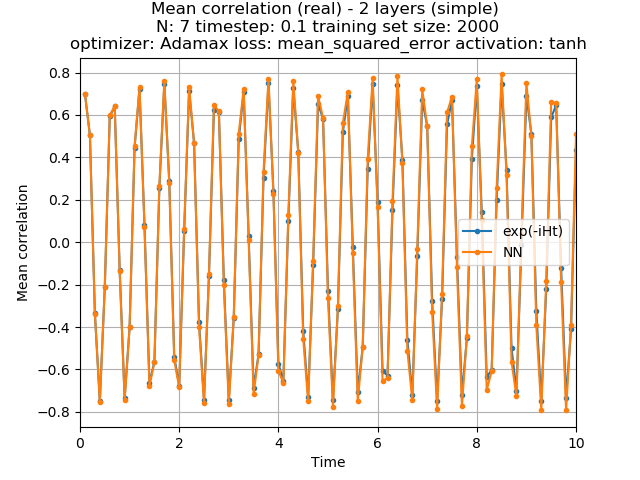
\includegraphics[scale=0.37]{./Searching_for_good_train_set_size/2_layers_simple_train_samples=2000_timestep=0.1_t_total=10.0_optimizer=Adamax_loss=mean_squared_error_activation=tanh/Corr_N=7_(real).png} \\ \hline

     3000 \\ (0.987) &
     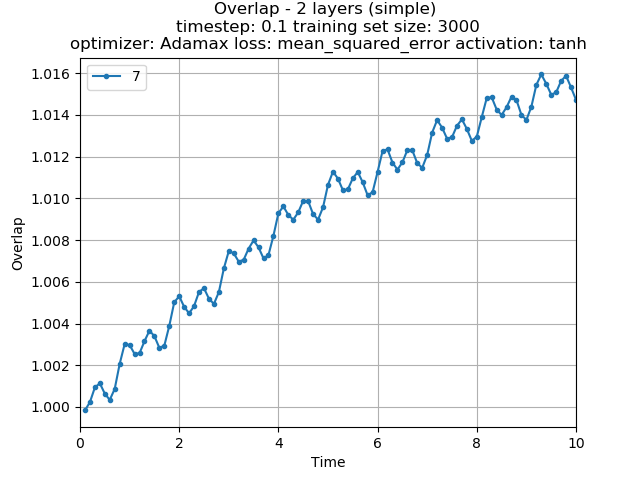
\includegraphics[scale=0.37]{./Searching_for_good_train_set_size/2_layers_simple_train_samples=3000_timestep=0.1_t_total=10.0_optimizer=Adamax_loss=mean_squared_error_activation=tanh/Overlap.png} &
     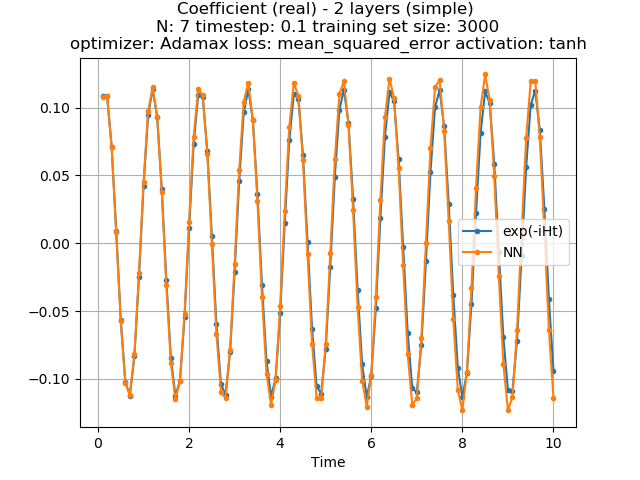
\includegraphics[scale=0.37]{./Searching_for_good_train_set_size/2_layers_simple_train_samples=3000_timestep=0.1_t_total=10.0_optimizer=Adamax_loss=mean_squared_error_activation=tanh/Coeff_N=7_(real).png} &
     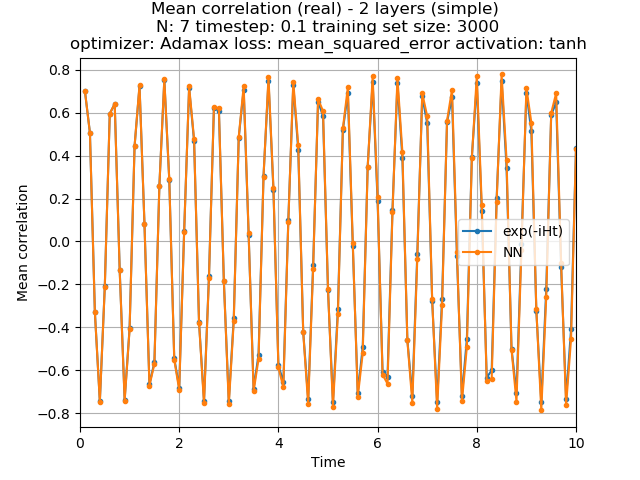
\includegraphics[scale=0.37]{./Searching_for_good_train_set_size/2_layers_simple_train_samples=3000_timestep=0.1_t_total=10.0_optimizer=Adamax_loss=mean_squared_error_activation=tanh/Corr_N=7_(real).png} \\ \hline

     4000 \\ (0.991) &
     \includegraphics[scale=0.37]{./Searching_for_good_train_set_size/2_layers_simple_train_samples=4000_timestep=0.1_t_total=10.0_optimizer=Adamax_loss=mean_squared_error_activation=tanh/Overlap.png} &
     \includegraphics[scale=0.37]{./Searching_for_good_train_set_size/2_layers_simple_train_samples=4000_timestep=0.1_t_total=10.0_optimizer=Adamax_loss=mean_squared_error_activation=tanh/Coeff_N=7_(real).png} &
     \includegraphics[scale=0.37]{./Searching_for_good_train_set_size/2_layers_simple_train_samples=4000_timestep=0.1_t_total=10.0_optimizer=Adamax_loss=mean_squared_error_activation=tanh/Corr_N=7_(real).png} \\ \hline

     5000 \\ (0.989) &
     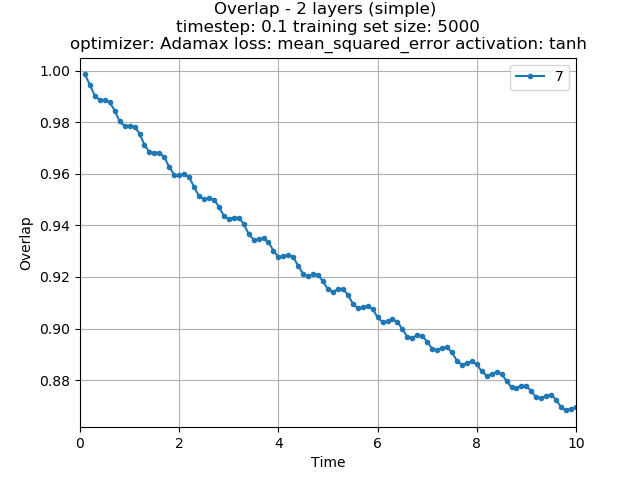
\includegraphics[scale=0.37]{./Searching_for_good_train_set_size/2_layers_simple_train_samples=5000_timestep=0.1_t_total=10.0_optimizer=Adamax_loss=mean_squared_error_activation=tanh/Overlap.png} &
     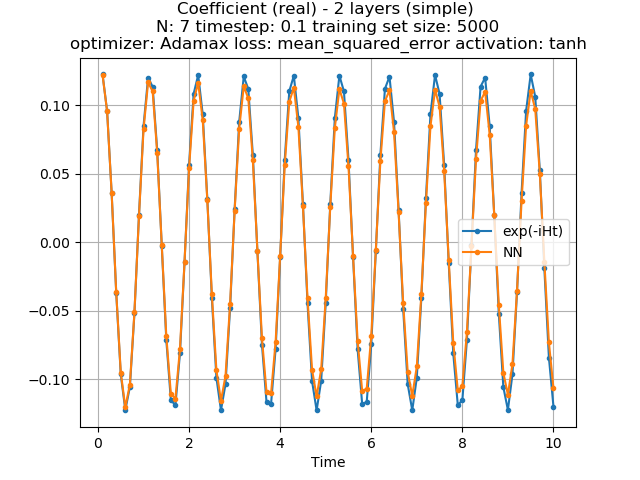
\includegraphics[scale=0.37]{./Searching_for_good_train_set_size/2_layers_simple_train_samples=5000_timestep=0.1_t_total=10.0_optimizer=Adamax_loss=mean_squared_error_activation=tanh/Coeff_N=7_(real).png} &
     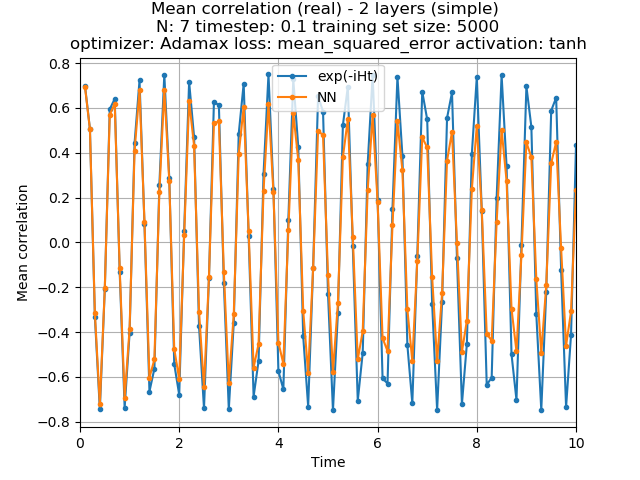
\includegraphics[scale=0.37]{./Searching_for_good_train_set_size/2_layers_simple_train_samples=5000_timestep=0.1_t_total=10.0_optimizer=Adamax_loss=mean_squared_error_activation=tanh/Corr_N=7_(real).png} \\ \hline

\end{tabular}

\subsection{Wnioski do tej sekcji}

\begin{itemize}
	\item Najlepsza precyzja występowała dla zbioru uczącego rozmiaru 400 000 (4000 losowych wektorów poddanych ewolucji). Wtedy tracimy na dokładności jedynie 0.008 dla całkowitego docelowego czasu ewolucji!
	\item Ciekawe jest to, że wystarczą 4000 losowe wektory, które są tylko poddawane ewolucji. Ponadto, takie wyniki są dużo lepsze niż dla 1 000 000 losowo wygenerowanych wektorów!
	\item Mimo "przetasowania" zbioru uczącego, wciąż dostajemy dobre rezultaty.
	\item Sieć dąży do takiej sytuacji, w której współczynnik będzie oscylował między około 0.1 a -0.1. Widać to najlepiej w przypadku z 4000 losowymi wektorami, tzn. późniejsze wartości współczynników są coraz bardziej "rozstrzelone". Miałem przykład, na którym było to lepiej widać, jednak pochopnie go usunąłem myśląc, że sieć się źle nauczyła...
\end{itemize}

\section{Sprawdzenie dokładności dla większej liczby warstw}

W tej sekcji chciałem sprawdzić, jak będzie sobie radziła sieć z takimi samymi parametrami jak ta z poprzedniej sekcji (Adamax, mean squared error, tanh), ale dla większej liczby warstw.

Tym razem w kolumnie z lewej oznaczonej jako \textbf{\#} podana jest liczba warstw w sieci (wszystkie wersje sieci uczone są na zbiorze uczącym złożonym z 400 000 wektorów, czyli było wygenerowanych 4000 wektorów losowych).

\begin{tabular}{|c|c|c|c|} \hline
     \# & Overlap & Korelacja & Współczynnik  \\ \hline
     1 \\ (0.994) &
     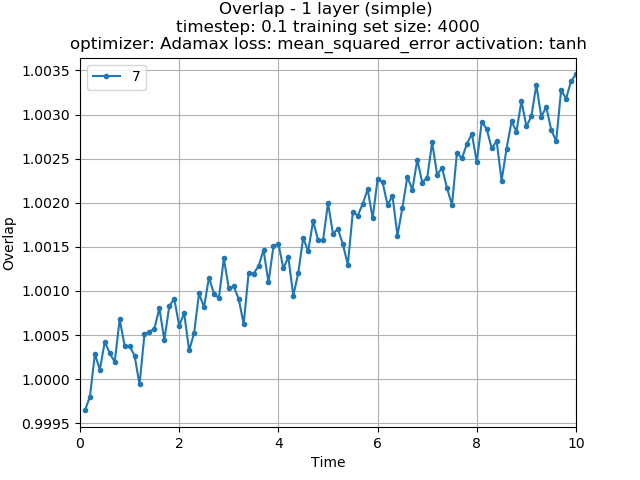
\includegraphics[scale=0.37]{./1_layer_simple_train_samples=4000_timestep=0.1_t_total=10.0_optimizer=Adamax_loss=mean_squared_error_activation=tanh/Overlap.png} &
     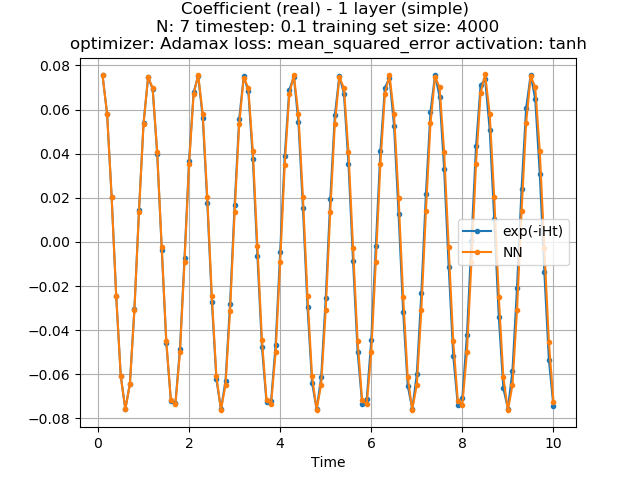
\includegraphics[scale=0.37]{./1_layer_simple_train_samples=4000_timestep=0.1_t_total=10.0_optimizer=Adamax_loss=mean_squared_error_activation=tanh/Coeff_N=7_(real).png} &
     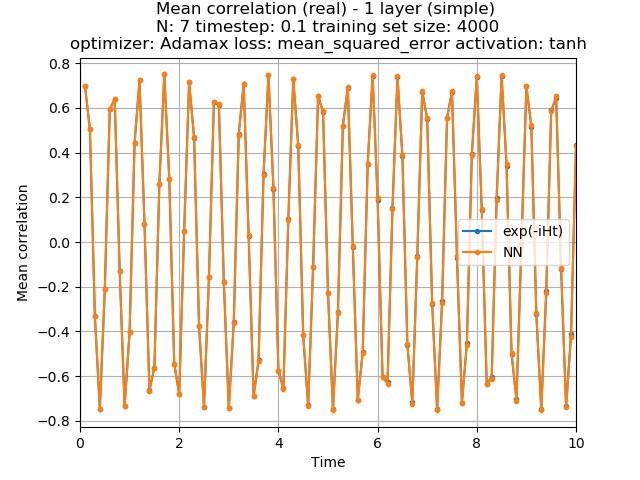
\includegraphics[scale=0.37]{./1_layer_simple_train_samples=4000_timestep=0.1_t_total=10.0_optimizer=Adamax_loss=mean_squared_error_activation=tanh/Corr_N=7_(real).png} \\ \hline

     2 \\ (0.991) &
     \includegraphics[scale=0.37]{./2_layers_simple_train_samples=4000_timestep=0.1_t_total=10.0_optimizer=Adamax_loss=mean_squared_error_activation=tanh/Overlap.png} &
     \includegraphics[scale=0.37]{./2_layers_simple_train_samples=4000_timestep=0.1_t_total=10.0_optimizer=Adamax_loss=mean_squared_error_activation=tanh/Coeff_N=7_(real).png} &
     \includegraphics[scale=0.37]{./2_layers_simple_train_samples=4000_timestep=0.1_t_total=10.0_optimizer=Adamax_loss=mean_squared_error_activation=tanh/Corr_N=7_(real).png} \\ \hline

     3 \\ (0.988) &
     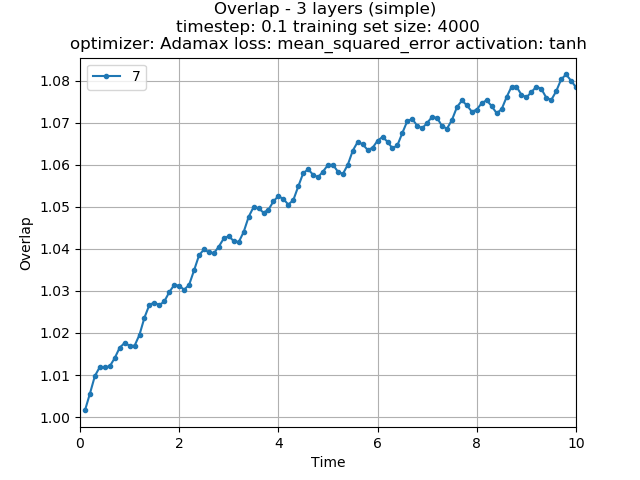
\includegraphics[scale=0.37]{./3_layers_simple_train_samples=4000_timestep=0.1_t_total=10.0_optimizer=Adamax_loss=mean_squared_error_activation=tanh/Overlap.png} &
     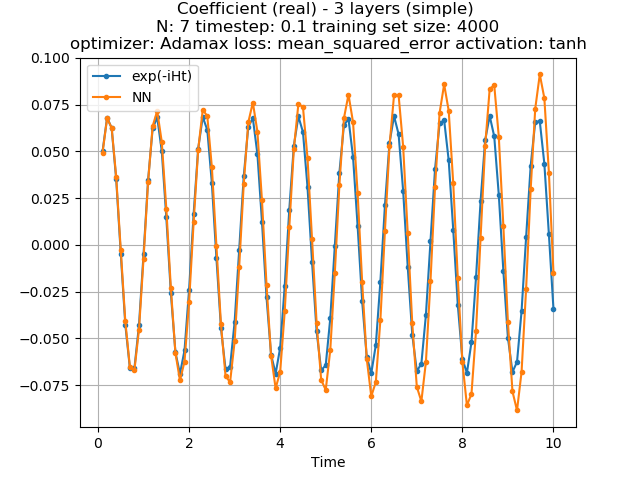
\includegraphics[scale=0.37]{./3_layers_simple_train_samples=4000_timestep=0.1_t_total=10.0_optimizer=Adamax_loss=mean_squared_error_activation=tanh/Coeff_N=7_(real).png} &
     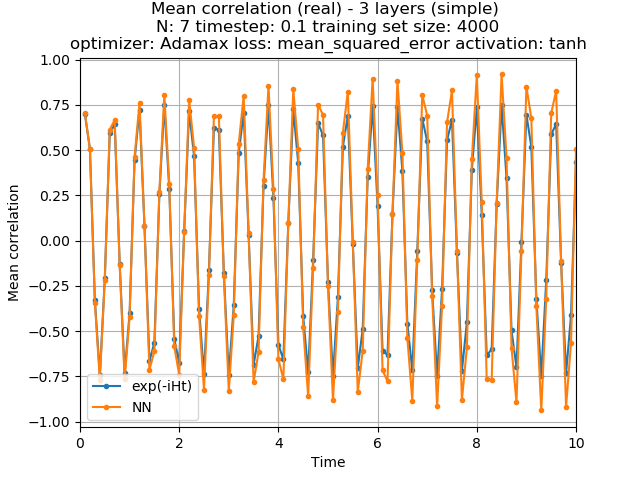
\includegraphics[scale=0.37]{./3_layers_simple_train_samples=4000_timestep=0.1_t_total=10.0_optimizer=Adamax_loss=mean_squared_error_activation=tanh/Corr_N=7_(real).png} \\ \hline

     4 \\ (0.925) &
     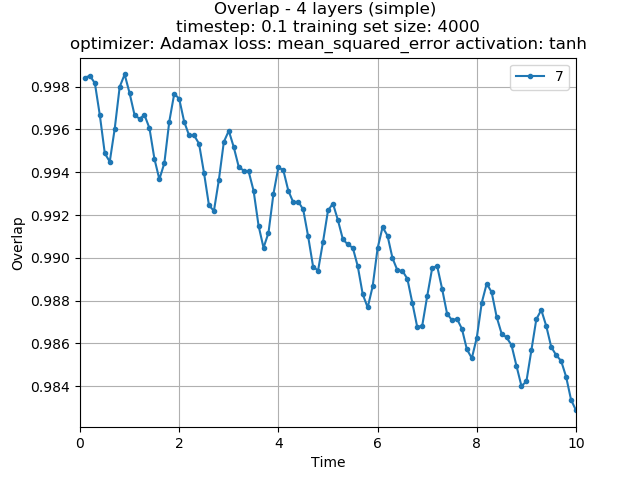
\includegraphics[scale=0.37]{./4_layers_simple_train_samples=4000_timestep=0.1_t_total=10.0_optimizer=Adamax_loss=mean_squared_error_activation=tanh/Overlap.png} &
     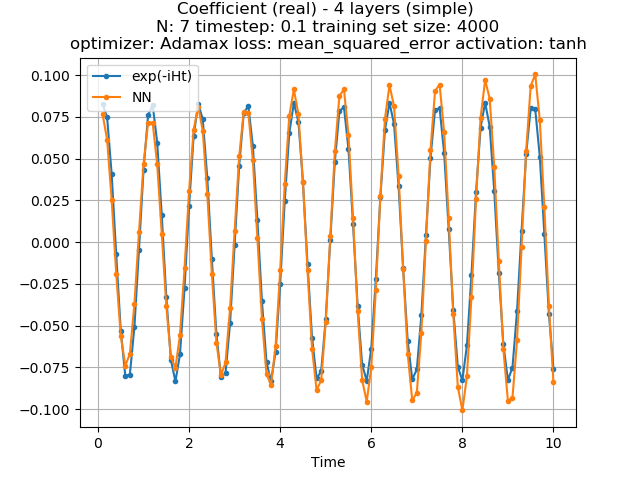
\includegraphics[scale=0.37]{./4_layers_simple_train_samples=4000_timestep=0.1_t_total=10.0_optimizer=Adamax_loss=mean_squared_error_activation=tanh/Coeff_N=7_(real).png} &
     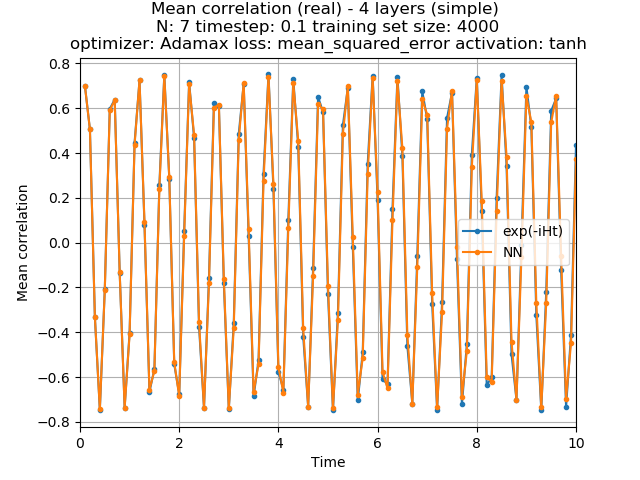
\includegraphics[scale=0.37]{./4_layers_simple_train_samples=4000_timestep=0.1_t_total=10.0_optimizer=Adamax_loss=mean_squared_error_activation=tanh/Corr_N=7_(real).png} \\ \hline

\end{tabular}


\begin{tabular}{|c|c|c|c|} \hline

     5 \\ (0.823) &
     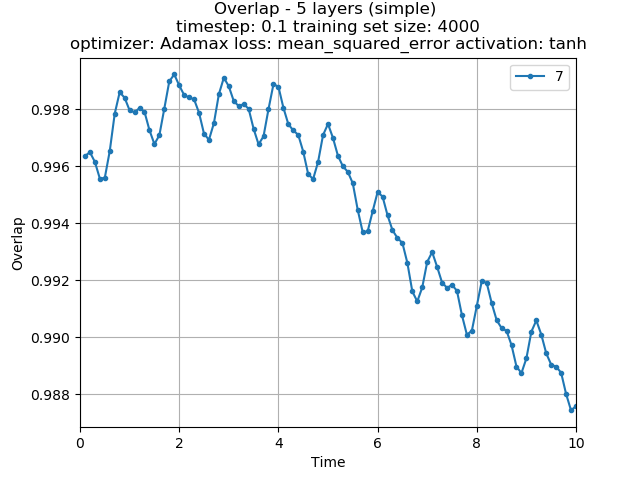
\includegraphics[scale=0.37]{./5_layers_simple_train_samples=4000_timestep=0.1_t_total=10.0_optimizer=Adamax_loss=mean_squared_error_activation=tanh/Overlap.png} &
     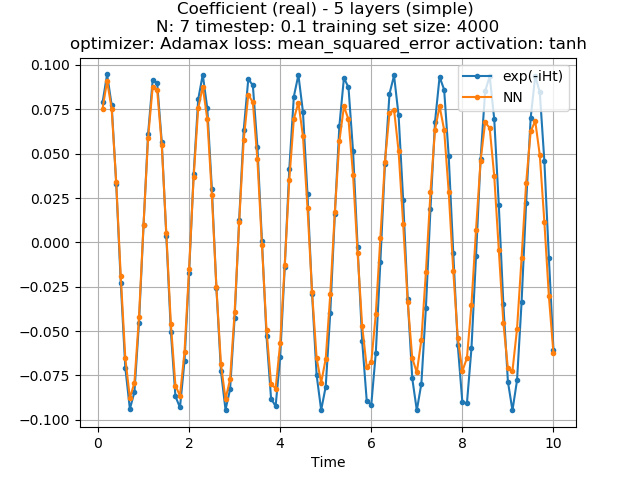
\includegraphics[scale=0.37]{./5_layers_simple_train_samples=4000_timestep=0.1_t_total=10.0_optimizer=Adamax_loss=mean_squared_error_activation=tanh/Coeff_N=7_(real).png} &
     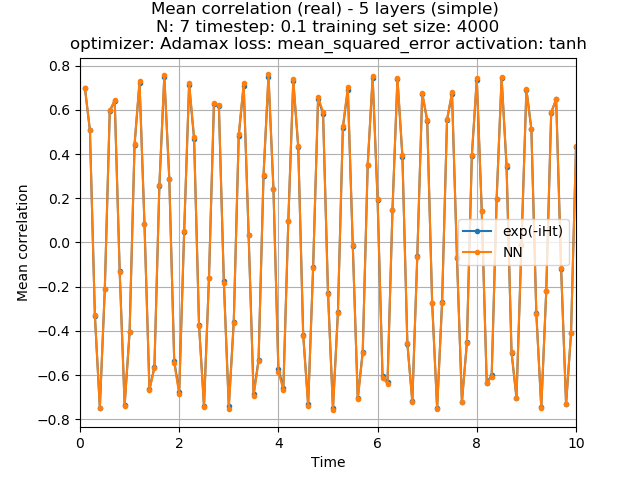
\includegraphics[scale=0.37]{./5_layers_simple_train_samples=4000_timestep=0.1_t_total=10.0_optimizer=Adamax_loss=mean_squared_error_activation=tanh/Corr_N=7_(real).png} \\ \hline

     6 \\ (0.738) &
     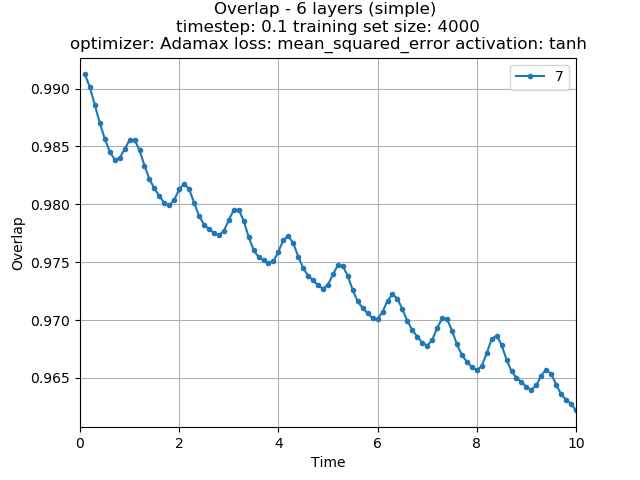
\includegraphics[scale=0.37]{./6_layers_simple_train_samples=4000_timestep=0.1_t_total=10.0_optimizer=Adamax_loss=mean_squared_error_activation=tanh/Overlap.png} &
     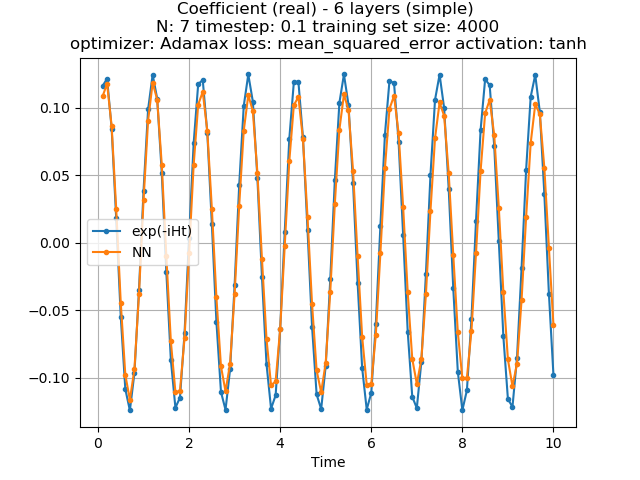
\includegraphics[scale=0.37]{./6_layers_simple_train_samples=4000_timestep=0.1_t_total=10.0_optimizer=Adamax_loss=mean_squared_error_activation=tanh/Coeff_N=7_(real).png} &
     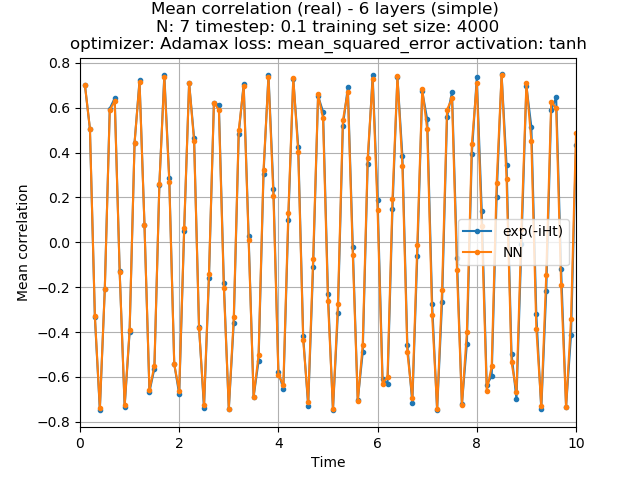
\includegraphics[scale=0.37]{./6_layers_simple_train_samples=4000_timestep=0.1_t_total=10.0_optimizer=Adamax_loss=mean_squared_error_activation=tanh/Corr_N=7_(real).png} \\ \hline

\end{tabular}

\subsection{Wnioski do tej sekcji:}
\begin{itemize}
	\item Co ciekawe, ciężko znaleźć bezpośrednie powiązanie między dokładnością sieci dla jednego kroku ewolucji a jej zachowaniem w dłuższej perspektywie. Tzn. np. sieć z 6 warstwami dla jednego kroku czasu miała dokładność wynoszącą ok. 74\%, ale overlap już dla tesowanej ewolucji utrzymywał się na poziomie powyżej 95\%.
\end{itemize}


\newpage
\section{Zbadanie zachowania dla sieci z dwoma warstwami, ale dłuższym całkowitym czasem ewolucji w trakcie ostatecznego testowania}

W tej sekcji chciałem sprawdzić, jak sieć ucząca się na wektorach dla całkowitej ewolucji wynoszącej maksymalnie 10 jednostek czasu poradzi sobie w dłuższej perspektywie, tzn. np. dla całkowitej ewolucji wynoszącej 20 i 30 jednostek.

Tym razem w lewej kolumnie oznaczonej jako \textbf{\#} podano mnożnik, przez jaki przemnożono docelowy całkowity czas ewolucji. Czyli w pierwszym wierszu są wyniki dla noramlnej ewolucji (10 jednostek czasu), w drugim dla 20 jednostek, a w 3 dla 30 jednostek.

\begin{tabular}{|c|c|c|c|} \hline
     \# & Overlap & Korelacja & Współczynnik  \\ \hline
     1x \\ (0.989) &
     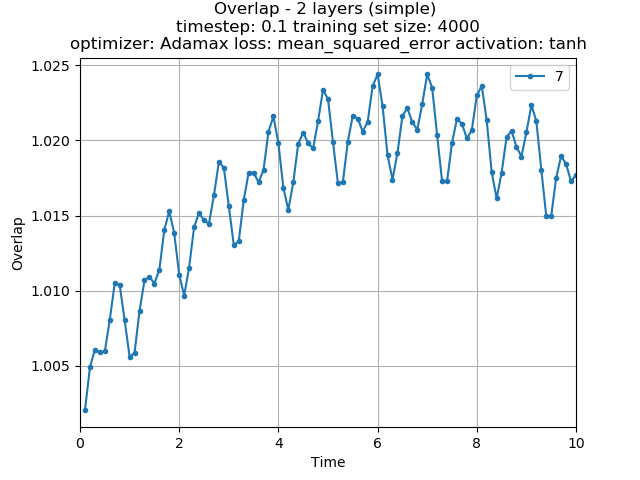
\includegraphics[scale=0.37]{./1,2,3x_longer_than_t_total/2_layers_simple_train_samples=4000_timestep=0.1_t_total=1x_optimizer=Adamax_loss=mean_squared_error_activation=tanh/Overlap.png} &
     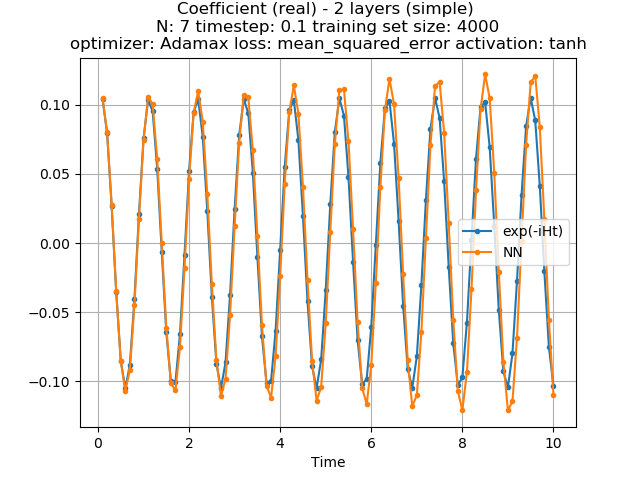
\includegraphics[scale=0.37]{./1,2,3x_longer_than_t_total/2_layers_simple_train_samples=4000_timestep=0.1_t_total=1x_optimizer=Adamax_loss=mean_squared_error_activation=tanh/Coeff_N=7_(real).png} &
     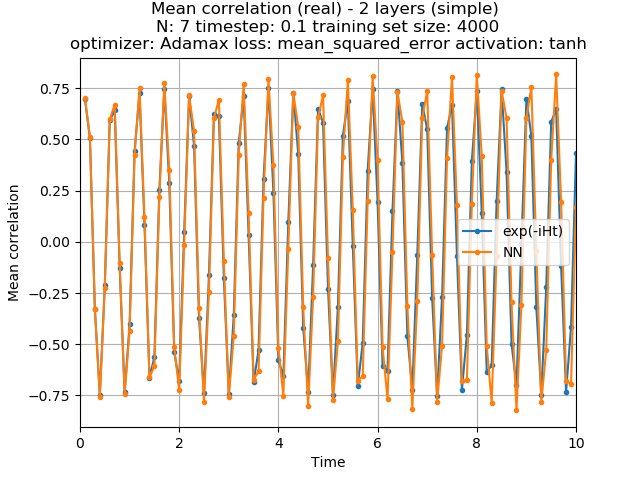
\includegraphics[scale=0.37]{./1,2,3x_longer_than_t_total/2_layers_simple_train_samples=4000_timestep=0.1_t_total=1x_optimizer=Adamax_loss=mean_squared_error_activation=tanh/Corr_N=7_(real).png} \\ \hline

     2x \\ (0.991) &
     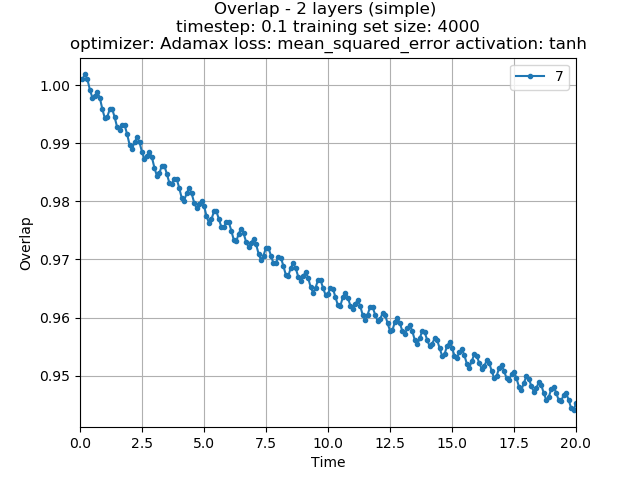
\includegraphics[scale=0.37]{./1,2,3x_longer_than_t_total/2_layers_simple_train_samples=4000_timestep=0.1_t_total=2x_optimizer=Adamax_loss=mean_squared_error_activation=tanh/Overlap.png} &
     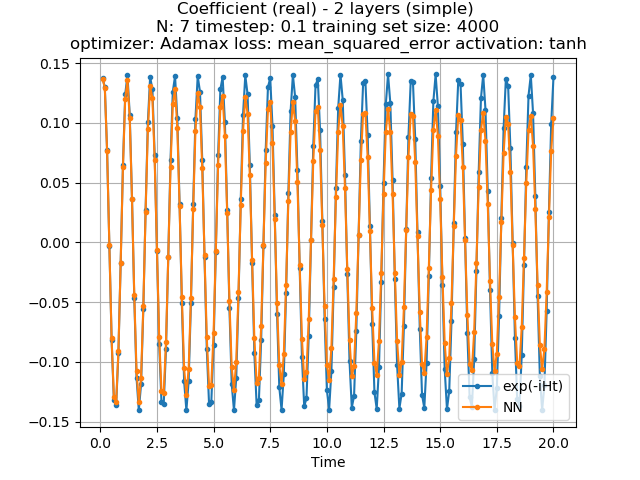
\includegraphics[scale=0.37]{./1,2,3x_longer_than_t_total/2_layers_simple_train_samples=4000_timestep=0.1_t_total=2x_optimizer=Adamax_loss=mean_squared_error_activation=tanh/Coeff_N=7_(real).png} &
     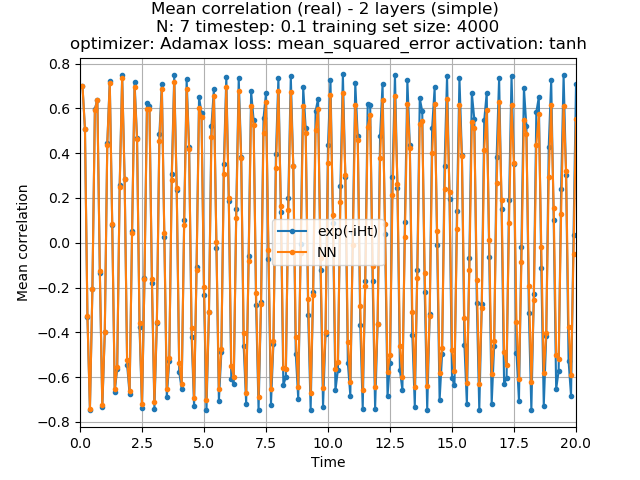
\includegraphics[scale=0.37]{./1,2,3x_longer_than_t_total/2_layers_simple_train_samples=4000_timestep=0.1_t_total=2x_optimizer=Adamax_loss=mean_squared_error_activation=tanh/Corr_N=7_(real).png} \\ \hline

	3x \\ (0.991) &
     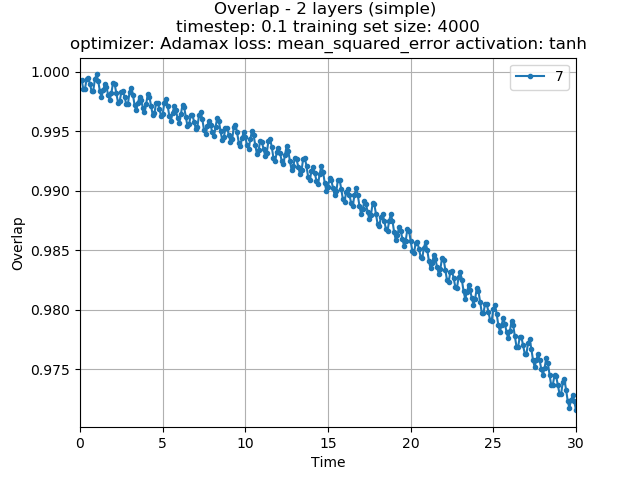
\includegraphics[scale=0.37]{./1,2,3x_longer_than_t_total/2_layers_simple_train_samples=4000_timestep=0.1_t_total=3x_optimizer=Adamax_loss=mean_squared_error_activation=tanh/Overlap.png} &
     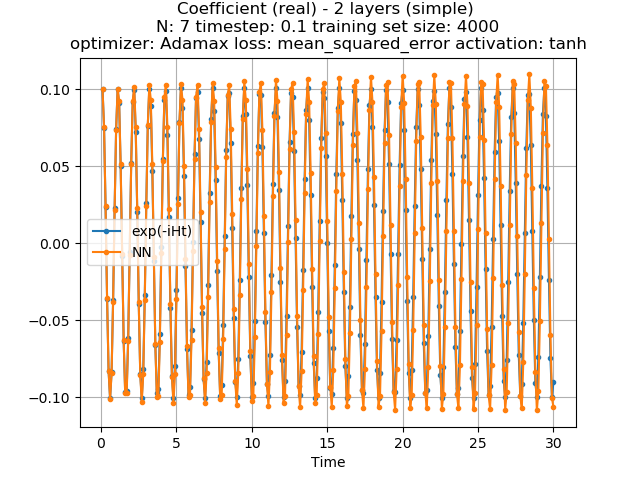
\includegraphics[scale=0.37]{./1,2,3x_longer_than_t_total/2_layers_simple_train_samples=4000_timestep=0.1_t_total=3x_optimizer=Adamax_loss=mean_squared_error_activation=tanh/Coeff_N=7_(real).png} &
     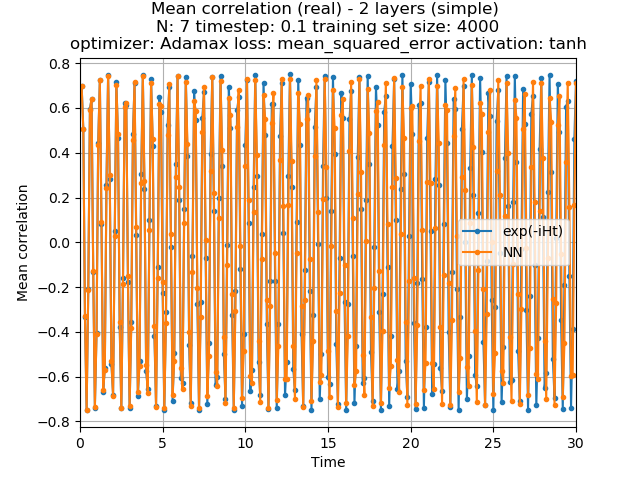
\includegraphics[scale=0.37]{./1,2,3x_longer_than_t_total/2_layers_simple_train_samples=4000_timestep=0.1_t_total=3x_optimizer=Adamax_loss=mean_squared_error_activation=tanh/Corr_N=7_(real).png} \\ \hline


\end{tabular}

\subsection{Wnioski do tej sekcji}

\begin{itemize}
	\item Sieć dość dobrze sobie radzi też dla dłuższych czasów ewolucji, niż te przewidziane w zbiorze uczącym.
\end{itemize}

\end{document}
